\documentclass[conference]{IEEEtran}
\IEEEoverridecommandlockouts
\usepackage{cite}
\usepackage{amsmath,amssymb,amsfonts}
\usepackage{graphicx}
\usepackage{textcomp}
\usepackage{xcolor}
\usepackage[T1]{fontenc}
\usepackage{tikz}
\usetikzlibrary{arrows.meta,positioning,fit,backgrounds}
\usepackage{booktabs}
\usepackage{array}

% hyperref va SIEMPRE al final de los paquetes; hidelinks evita el recuadro de color
\usepackage[hidelinks,breaklinks=true]{hyperref}
\urlstyle{tt}

% Rotulos en espanol (sin babel, para no alterar el formato IEEE)
\renewcommand{\tablename}{TABLA}
\renewcommand{\figurename}{Fig.}

\begin{document}

\title{Hermes-SOC: Un Framework Multiagente para la Detección Diferenciada,
Mitigación y Documentación de Fallas y Ataques Cibernéticos en Servicios y
Microservicios}

\author{\IEEEauthorblockN{Leonardo Andrés Rodríguez Lagos}
\IEEEauthorblockA{\textit{Dep. Ingeniería Civil Informática} \\
\textit{Universidad de Tarapacá}\\
Arica, Chile \\
leonardo.rodriguez.lagos@alumnos.uta.cl}
}

\maketitle

\begin{abstract}
Los servidores y arquitecturas de microservicios pueden degradarse por dos causas
de naturaleza distinta: fallas operativas comunes o ataques cibernéticos activos.
Diferenciar ambas causas, aplicar la contramedida correcta y documentar lo ocurrido
son hoy tareas manuales y secuenciales. En este trabajo se presenta Hermes-SOC, un
sistema multiagente construido sobre Hermes Agent, en el que tres agentes
especializados se comunican mediante el protocolo Agent-to-Agent (A2A): un agente de
Detección que clasifica el evento a partir de métricas y registros, un agente de
Mitigación que ejecuta la contramedida correspondiente mediante herramientas MCP, y
un agente de Documentación que genera el reporte técnico del incidente. Los tres
agentes comparten un mismo modelo local y se diferencian únicamente por su prompt de
rol y por las herramientas a las que acceden, sin entrenamiento adicional. El sistema
fue implementado sobre un banco de pruebas en contenedores y evaluado en cuatro
escenarios inyectados (falla de latencia, DDoS de capa de aplicación, fuerza bruta y
operación normal) bajo dos condiciones: la cadena multiagente y un agente único que
ejecuta las tres fases. En un piloto de 40 corridas se observó que la clasificación fue correcta en el
89\,\% de las corridas con respuesta en la condición multiagente y en el 100\,\% en la
de agente único, sin falsas alarmas en el escenario normal. Sin embargo, el agente
único completó la tarea en solo 7 de 20 corridas, frente a 18 de 20 de la cadena
multiagente, al agotar de forma sistemática el tope de tiempo de la plataforma. Se
detectaron además discrepancias entre las acciones declaradas y las ejecutadas en 13
de las 40 corridas.
\end{abstract}

\begin{IEEEkeywords}
sistemas multiagente, operaciones de seguridad, respuesta a incidentes, mitigación
de DDoS, agentes basados en modelos de lenguaje de gran escala
\end{IEEEkeywords}

\section{Contexto y Problema}
En entornos de producción, un servicio o microservicio puede dejar de responder
correctamente por motivos muy distintos entre sí: una falla operativa común (falta
de memoria, un proceso caído, una dependencia externa lenta) o un ataque cibernético
activo, siendo el más frecuente y disruptivo la denegación de servicio distribuida
(DDoS). El tratamiento correcto de cada caso es fundamentalmente diferente: una
falla operativa se resuelve reiniciando o escalando el recurso afectado, mientras
que un ataque requiere contención activa (bloqueo de direcciones IP, limitación de
tasa de peticiones, aislamiento del servicio).

Actualmente este diagnóstico diferencial lo realiza un analista humano revisando
tableros y registros, lo cual introduce demoras críticas, un problema ampliamente
documentado en la literatura de automatización de Centros de Operaciones de
Seguridad (SOC) mediante inteligencia artificial \cite{khayat2025}. Trabajos
recientes han explorado marcos multiagente jerárquicos para el diagnóstico de causa
raíz en microservicios \cite{kataria2025}, y otra línea se ha enfocado en la
automatización del SOC mediante agentes de modelos de lenguaje \cite{srinivas2025,
saju2026}. Sin embargo, estos enfoques abordan una sola fase por separado:
diagnóstico de rendimiento o respuesta de seguridad, y pocos incorporan validación
estructural o razonamiento de riesgo antes de ejecutar una acción de contención
\cite{roy2026}. Existe entonces un vacío en sistemas que integren la clasificación
diferencial junto con una mitigación y documentación adaptadas a esa clasificación.

\section{Solución Propuesta}
Se propone Hermes-SOC, un flujo multiagente sobre Hermes Agent compuesto por tres
agentes especializados que se comunican mediante el protocolo A2A. El agente de
\textbf{Detección} consume métricas y registros de acceso y determina si la anomalía
corresponde a una falla operativa o a un ataque activo, entregando la clasificación,
su nivel de confianza y la evidencia que la sustenta. El agente de
\textbf{Mitigación} recibe esa clasificación y ejecuta la contramedida
correspondiente mediante herramientas conectadas por MCP, evaluando el impacto
operativo de cada acción antes de aplicarla \cite{roy2026}. El agente de
\textbf{Documentación} recibe la evidencia acumulada y redacta un reporte técnico
que responde qué se detectó, cómo se detectó, qué acción se tomó y qué se recomienda
para prevenir la recurrencia.

\begin{figure*}[t]
\centering
\resizebox{\textwidth}{!}{%
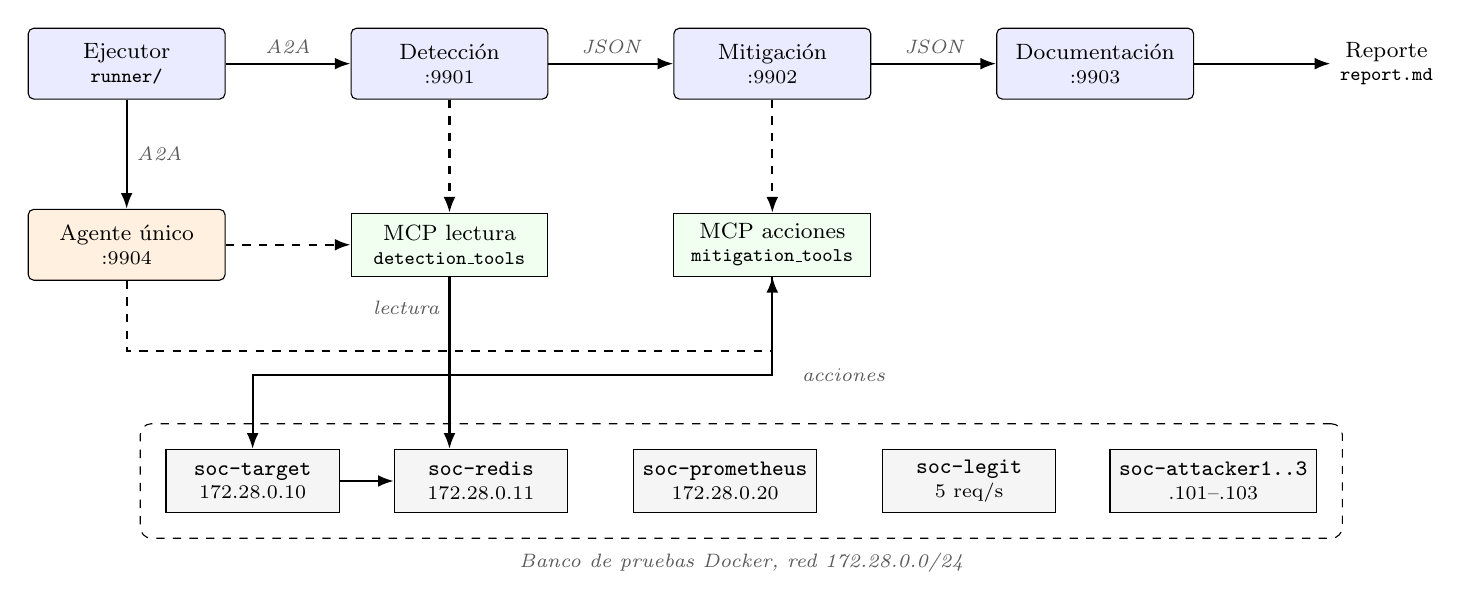
\begin{tikzpicture}[
  font=\footnotesize,
  agente/.style={draw, rounded corners=2pt, minimum height=9mm, minimum width=25mm,
                 align=center, fill=blue!8},
  tool/.style={draw, minimum height=8mm, minimum width=25mm, align=center,
               fill=green!6},
  infra/.style={draw, minimum height=8mm, minimum width=22mm, align=center,
                fill=black!4},
  flecha/.style={-{Latex[length=2mm]}, thick},
  nota/.style={font=\scriptsize\itshape, text=black!65}
]
  % --- cadena A2A ---
  \node[agente] (ej)  at (0,0)    {Ejecutor\\[-1pt]\scriptsize\texttt{runner/}};
  \node[agente] (det) at (4.1,0)  {Detección\\[-1pt]\scriptsize:9901};
  \node[agente] (mit) at (8.2,0)  {Mitigación\\[-1pt]\scriptsize:9902};
  \node[agente] (doc) at (12.3,0) {Documentación\\[-1pt]\scriptsize:9903};
  \node[align=center] (rep) at (16.0,0) {Reporte\\[-1pt]\scriptsize\texttt{report.md}};

  \draw[flecha] (ej)  -- node[above, nota] {A2A}  (det);
  \draw[flecha] (det) -- node[above, nota] {JSON} (mit);
  \draw[flecha] (mit) -- node[above, nota] {JSON} (doc);
  \draw[flecha] (doc) -- (rep);

  % --- agente unico ---
  \node[agente, fill=orange!12] (uni) at (0,-2.3)
       {Agente único\\[-1pt]\scriptsize:9904};
  \draw[flecha] (ej) -- node[right, nota] {A2A} (uni);

  % --- herramientas MCP ---
  \node[tool] (mcp1) at (4.1,-2.3)
       {MCP lectura\\[-1pt]\scriptsize\texttt{detection\_tools}};
  \node[tool] (mcp2) at (8.2,-2.3)
       {MCP acciones\\[-1pt]\scriptsize\texttt{mitigation\_tools}};
  \draw[flecha, dashed] (det) -- (mcp1);
  \draw[flecha, dashed] (mit) -- (mcp2);
  \draw[flecha, dashed] (uni) -- (mcp1);
  \draw[flecha, dashed] (uni.south) -- (0,-3.65) -- (8.2,-3.65) -- (mcp2.south);

  % --- banco de pruebas ---
  \node[infra] (target) at (1.6,-5.3) {\texttt{soc-target}\\[-1pt]\scriptsize 172.28.0.10};
  \node[infra] (redis)  at (4.5,-5.3) {\texttt{soc-redis}\\[-1pt]\scriptsize 172.28.0.11};
  \node[infra] (prom)   at (7.6,-5.3) {\texttt{soc-prometheus}\\[-1pt]\scriptsize 172.28.0.20};
  \node[infra] (legit)  at (10.7,-5.3) {\texttt{soc-legit}\\[-1pt]\scriptsize 5 req/s};
  \node[infra] (atk)    at (13.8,-5.3) {\texttt{soc-attacker1..3}\\[-1pt]\scriptsize .101--.103};

  \draw[flecha] (mcp1.south) -- node[pos=0.18, left, nota] {lectura} (prom.north -| mcp1);
  \draw[flecha] (mcp2.south) -- ++(0,-1.25) -| (target.north);
  \node[nota, anchor=west] at (8.45,-3.95) {acciones};
  \draw[flecha] (target) -- (redis);

  \begin{scope}[on background layer]
    \node[draw, dashed, rounded corners, fit=(target)(redis)(prom)(legit)(atk),
          inner sep=3.2mm] (bp) {};
  \end{scope}
  \node[nota, below=0.5mm of bp] {Banco de pruebas Docker, red 172.28.0.0/24};
\end{tikzpicture}}
\caption{Arquitectura de Hermes-SOC. El ejecutor transporta el resultado de cada
agente al siguiente mediante mensajes A2A independientes; la condición de agente
único resuelve las tres fases en un solo perfil. Las herramientas MCP de detección
son de solo lectura y las de mitigación ejecutan acciones acotadas y auditadas sobre
el banco de pruebas.}
\label{fig:arq}
\end{figure*}

\section{Metodología}
\subsection{Diseño experimental}
Se empleó un diseño factorial de cuatro escenarios por dos condiciones. Los
escenarios correspondieron a una falla operativa de latencia, un ataque DDoS de capa
de aplicación, un ataque de fuerza bruta y una condición de operación normal
destinada a medir falsos positivos. Las condiciones correspondieron a la cadena
multiagente de tres perfiles y a un agente único que resolvió las tres fases. El
orden de ejecución fue aleatorizado por bloques. Se ejecutaron cinco repeticiones por
celda, lo que totaliza 40 corridas. En el escenario de falla la variante fue rotada
entre latencia, agotamiento de memoria e indisponibilidad de la dependencia, de modo
que las cinco repeticiones cubrieran los tres modos de fallo. Por el costo de cómputo
de cada corrida, del orden de minutos, el tamaño de muestra sigue siendo reducido y
los intervalos se interpretan como preliminares.

\subsection{Banco de pruebas}
El banco de pruebas fue desplegado sobre Docker en una red fija
\texttt{172.28.0.0/24}, aislada del resto del equipo, y su composición se muestra en
la Fig.~\ref{fig:arq}. El servicio objetivo fue una aplicación FastAPI que expuso
los extremos \texttt{/}, \texttt{/health}, \texttt{/api/data} (dependiente de
Redis), \texttt{/login} (con derivación PBKDF2, deliberadamente costosa) y
\texttt{/metrics}. Cada petición fue registrada como una línea JSON con marca de
tiempo, dirección IP, método, ruta, código de estado y latencia. Un contenedor
generador de tráfico legítimo sostuvo una carga base de 5 peticiones por segundo
durante todos los escenarios, de modo que la carga legítima estuvo siempre presente
y permitió medir el bloqueo indebido.

\subsection{Configuración experimental}
La configuración de hardware y software utilizada se detalla en la
Tabla~\ref{tab:setup}. Los cuatro perfiles de agente emplearon el mismo modelo, de
modo que las diferencias observadas entre condiciones no fueran atribuibles al
modelo. La longitud de contexto fue fijada en 64\,000 tokens porque Hermes Agent
rechaza modelos con un contexto efectivo menor; un modelo de 8B evaluado inicialmente
fue descartado por esta razón.

\begin{table}[htbp]
\caption{Configuración de hardware y software}
\begin{center}
\footnotesize
\begin{tabular}{@{}ll@{}}
\toprule
\textbf{Componente} & \textbf{Detalle} \\
\midrule
Equipo & Intel i9-14900HX, 32 GB RAM \\
GPU & NVIDIA RTX 5070 Laptop, 8 GB VRAM \\
Sistema operativo & Windows con WSL2 \\
Hermes Agent & v0.21.5+4108.g105568c (nativo) \\
Ollama & 0.40.11 \\
Modelo & \texttt{qwen3.5:9b} (4 perfiles) \\
Contexto & 64\,000 tokens; 30\,\%/70\,\% CPU/GPU \\
Variables Ollama & \texttt{FLASH\_ATTENTION=1}, \texttt{KV\_CACHE\_TYPE=q8\_0}, \\
 & \texttt{NUM\_PARALLEL=1}, \texttt{KEEP\_ALIVE=-1} \\
Contenedores & Docker Desktop (WSL2), red 172.28.0.0/24 \\
Python & 3.14; \texttt{mcp} 2.3.0 \\
Puertos A2A & 9901--9904 \\
\bottomrule
\end{tabular}
\label{tab:setup}
\end{center}
\end{table}

\subsection{Inyección de escenarios}
Cada escenario fue inyectado por un módulo que registró su etiqueta real y sus
parámetros en un archivo \texttt{ground\_truth.json}, el cual constituyó la verdad
de referencia contra la que se evaluó la clasificación. Las fallas fueron
introducidas mediante tres mecanismos: latencia artificial con \texttt{tc netem},
agotamiento de memoria con \texttt{stress-ng} e indisponibilidad de la dependencia
mediante la detención del contenedor de Redis. El DDoS fue
generado desde tres contenedores atacantes con 100 conexiones concurrentes por
origen. La fuerza bruta fue generada desde un único origen contra el extremo de
autenticación. Las firmas observadas para cada escenario, medidas en ventanas de
30 s, se resumen en la Tabla~\ref{tab:firmas}. Las fallas persistieron hasta ser
corregidas; los ataques tuvieron duración acotada.

\begin{table}[htbp]
\caption{Firmas observadas por escenario (ventana de 30 s)}
\begin{center}
\footnotesize
\begin{tabular}{@{}lrrr>{\raggedright\arraybackslash}p{1.75cm}@{}}
\toprule
\textbf{Escenario} & \textbf{Tasa} & \textbf{IP} & \textbf{p95} & \textbf{Señal} \\
 & \textbf{(req/s)} & \textbf{únicas} & \textbf{(ms)} & \textbf{distintiva} \\
\midrule
Base          & 5    & 1 & 0.6     & --- \\
Latencia      & 5    & 1 & 813     & sin cambio de carga \\
Memoria       & 5    & 1 & 11      & memoria 0.89 \\
Redis caído   & 5    & 1 & 15\,000 & 16\,\% de 5xx \\
DDoS          & 1145 & 4 & 243     & 3 IP, $\approx$33\,\% c/u \\
Fuerza bruta  & 80   & 2 & ---     & 99.7\,\% de 401 \\
\bottomrule
\end{tabular}
\label{tab:firmas}
\end{center}
\end{table}

\subsection{Configuración de los agentes}
Los agentes no fueron entrenados. Se empleó el mismo modelo base en las dos
condiciones, sin ajuste fino, sin modificación de pesos y sin base de conocimiento
externa, de modo que el comportamiento de cada agente quedó determinado
exclusivamente por su configuración en tiempo de inferencia. Esta configuración
constó de tres elementos: un prompt de rol que fijó el procedimiento, los criterios
orientativos de clasificación, el formato de salida en JSON y la prohibición de
declarar datos no observados; el conjunto de herramientas MCP accesible, que delimitó
qué pudo observar y qué pudo ejecutar cada agente; y el mensaje de disparo con el que
el ejecutor inició cada tarea y transportó el resultado al siguiente agente.

En la condición multiagente, cada uno de los tres agentes dispuso de su propio prompt
y de un subconjunto acotado de herramientas. En la condición de agente único, el mismo
modelo recibió un prompt que cubrió las tres fases y la totalidad de las herramientas.
En consecuencia, la variable manipulada fue la arquitectura y el reparto del trabajo,
y no el modelo ni su capacidad.

\subsection{Herramientas y salvaguardas}
El agente de Detección dispuso únicamente de herramientas de solo lectura, que
entregaron resúmenes agregados de tráfico, estado de contenedores y muestras de
registro, en lugar de registros crudos. El agente de Mitigación dispuso de un
conjunto acotado de acciones: reinicio de servicio, bloqueo de dirección IP,
limitación de tasa, listado de reglas de cortafuegos y verificación de recuperación.
Se implementaron tres salvaguardas: una lista de direcciones protegidas que no
pueden ser bloqueadas, la restricción del reinicio a los dos contenedores del banco
de pruebas, y el registro de toda acción ejecutada en una bitácora de auditoría
independiente de lo que el agente declara haber hecho. Esta última salvaguarda
permitió medir la discrepancia entre acciones declaradas y ejecutadas, una
precaución recomendada para agentes con capacidad de ejecución \cite{hu2026,
debenedetti2026}.

\subsection{Procedimiento experimental}
Cada corrida siguió un procedimiento fijo de cinco fases. En la primera fase el
banco de pruebas fue restablecido a su estado base y verificado mediante una rutina
de comprobación que valida la disponibilidad del servicio, de Redis, de Prometheus y
de las utilidades de inyección dentro del contenedor. En la segunda fase se inyectó
el escenario correspondiente y se registró su etiqueta real. Posteriormente, en la
tercera fase, el ejecutor invocó la cadena multiagente o el agente único según la
condición asignada. Durante la cuarta fase un monitor independiente consultó el
estado del servicio cada 5 s hasta constatar la recuperación o agotar la ventana de
observación. Finalmente, en la quinta fase se consolidaron la traza de la corrida,
el reporte generado y la fila de métricas correspondiente. El ejecutor fue diseñado
para ser reanudable, de modo que una interrupción no invalida las corridas previas.

\subsection{Reproducibilidad}
El código del banco de pruebas, de los agentes, de las herramientas MCP, del ejecutor
y del análisis fue publicado en un repositorio de acceso abierto\footnote{Disponible
en \url{https://github.com/TheShac/hermes-soc}.} junto con el archivo de
dependencias y la definición de los contenedores, de manera que el entorno puede ser
reconstruido sin intervención manual. Los prompts de rol de los cuatro perfiles, las
rutinas de inyección de escenarios, la rutina de verificación del banco de pruebas y
el procedimiento de análisis se encuentran igualmente versionados. Las trazas crudas
de cada corrida fueron conservadas y las tablas de métricas consolidadas se
distribuyen con el repositorio, por lo que los valores reportados pueden ser
recalculados de forma independiente.

\subsection{Métricas e instrumentación}
Se registraron las siguientes métricas por corrida. El acierto de clase y de
subtipo fueron determinados comparando la salida del agente de Detección contra la
verdad de referencia. El tiempo hasta la detección fue medido solo en la condición
multiagente, donde existe un salto de Detección observable. El tiempo hasta la
primera acción y el tiempo hasta la recuperación (MTTR) fueron medidos en ambas
condiciones por un monitor independiente que consultó el estado del servicio cada
5 s, de modo que la recuperación fue verificada contra el servicio y no contra lo
declarado por los agentes. Se contabilizaron además las acciones ejecutadas, las
acciones sobre direcciones IP incorrectas, las acciones innecesarias y los
reintentos de formato, admitiéndose como máximo un reintento por salto en ambas
condiciones.

\subsection{Desviación respecto del diseño original}
La propuesta original planteaba que los agentes se invocaran entre sí. Durante la
implementación se verificó que la llamada entre agentes impone un tiempo máximo fijo
de 120 s, mientras que cada agente requirió entre 100 y 200 s con el modelo local.
En consecuencia, el ejecutor transportó el resultado de cada agente al siguiente.
Cada salto siguió siendo un mensaje A2A real, pero la decisión de a qué agente
invocar no fue tomada por el agente. Esta desviación se aplicó por igual a ambas
condiciones, por lo que no favorece a ninguna.

Se constató asimismo que la plataforma de agentes interrumpe toda tarea que supere los
300 s, con independencia del tiempo máximo configurado en el ejecutor, que fue fijado
en 900 s por salto. Dicho tope no fue impuesto por el diseño experimental y resultó
determinante en los resultados, por lo que se registró como una variable observada.

\section{Resultados}
Se completaron las 40 corridas previstas. Los resultados agregados por escenario y
condición se presentan en la Tabla~\ref{tab:resultados}.

\subsection{Fiabilidad de respuesta}
En la Fig.~\ref{fig:desenlace} se observa que el desenlace de cada corrida estuvo
dominado por un factor no previsto en el diseño: la capacidad del sistema de emitir
una respuesta. La condición multiagente produjo una salida estructurada válida en 18
de 20 corridas (90\,\%), mientras que el agente único lo hizo en 7 de 20 (35\,\%). En
las corridas restantes la tarea A2A terminó en estado fallido tras 300 s sin devolver
contenido: 11 corridas del agente único y 3 de la cadena multiagente. La mediana de
duración de la cadena fue de 116.6 s en la condición multiagente y de 300.1 s en la
de agente único, valor este último que coincide con el tope de la plataforma.

Esto indica que el límite no fue alcanzado por azar, sino que el agente único lo
agotó de forma sistemática. Dicho agente debió resolver las tres fases dentro de un
mismo contexto y con la totalidad de las herramientas declaradas, lo que elevó tanto
la longitud del contexto como el número de invocaciones del modelo por tarea. Por
consiguiente, la especialización en agentes no actuó aquí como una optimización del
desempeño, sino como la condición que permitió que la tarea cupiera dentro del
presupuesto de tiempo de la plataforma.

\begin{figure}[htbp]
\centerline{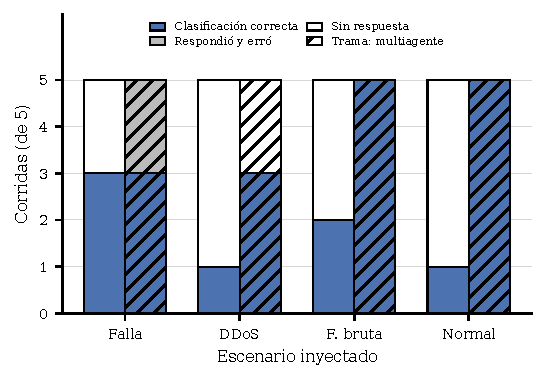
\includegraphics[width=\columnwidth]{fig/desenlace.pdf}}
\caption{Desenlace de las corridas por escenario y condición. Las barras sin trama
corresponden al agente único y las tramadas a la cadena multiagente. El segmento
blanco indica las corridas en que la tarea expiró sin devolver una salida
estructurada.}
\label{fig:desenlace}
\end{figure}

\subsection{Clasificación diferencial}
Al restringir el análisis a las corridas que sí respondieron, la clasificación fue
correcta en el 89\,\% de los casos en la condición multiagente y en el 100\,\% en la
de agente único. En otras palabras, el agente único no se equivocó cuando respondió;
lo que ocurrió es que respondió en poco más de un tercio de las corridas. Sobre el
total de corridas, la clase fue correcta en 16 de 20 con la cadena multiagente y en 7
de 20 con el agente único.

La matriz de confusión de la condición multiagente se presenta en la
Tabla~\ref{tab:confusion}. Los dos errores de clase se produjeron en el escenario de
falla por agotamiento de memoria: en una corrida el sistema informó un estado sano
pese a la degradación, y en otra atribuyó la falla a un ataque. A ellos se suma una
confusión de subtipo en la que una caída de la dependencia fue informada como falla
de latencia, lo que resulta coherente con la firma observada, ya que la indisponibilidad
de Redis eleva la latencia percibida. No se registró ninguna falsa alarma en el
escenario normal en ninguna de las dos condiciones.

\begin{table}[htbp]
\caption{Matriz de confusión del subtipo, condición multiagente}
\begin{center}
\footnotesize
\setlength{\tabcolsep}{3.4pt}
\begin{tabular}{@{}lcccccc@{}}
\toprule
\textbf{Real $\downarrow$} & \textbf{F. bruta} & \textbf{DDoS} & \textbf{Lat.} &
\textbf{Mem.} & \textbf{Ning.} & \textbf{S/r} \\
\midrule
Fuerza bruta  & \textbf{5} & 0 & 0 & 0 & 0 & 0 \\
DDoS          & 0 & \textbf{3} & 0 & 0 & 0 & 2 \\
Latencia      & 0 & 0 & \textbf{2} & 0 & 0 & 0 \\
Memoria       & 0 & 0 & 0 & \textbf{1} & 1 & 0 \\
Dependencia   & 0 & 0 & 1 & 0 & 0 & 0 \\
Ninguno       & 0 & 0 & 0 & 0 & \textbf{5} & 0 \\
\bottomrule
\multicolumn{7}{l}{\scriptsize S/r: la tarea expiró sin devolver una salida
estructurada.} \\
\end{tabular}
\label{tab:confusion}
\end{center}
\end{table}

\subsection{Tiempos de respuesta}
Los tiempos se desglosan en la Fig.~\ref{fig:mttr}. Como se indica en dicha figura,
el tiempo total hasta la recuperación estuvo dominado por el tiempo hasta la primera
acción y no por la recuperación posterior del servicio, que se completó en menos de
30 s en todas las celdas. Por consiguiente, el costo del sistema se concentra en la
inferencia del modelo y no en la infraestructura.

El tiempo medio hasta la primera acción fue de 79.4 s en la condición multiagente
($n=11$) y de 132.8 s en la de agente único ($n=10$). El MTTR medio fue, en cambio,
de 114.5 s y 104.9 s respectivamente, sin diferencia apreciable. No obstante, esta
última comparación debe leerse con cautela: solo admite las corridas en que hubo
mitigación medible, que son la mayoría en la condición multiagente y una minoría en
la de agente único, por lo que compara el mejor caso del agente único contra el caso
típico de la cadena. El tiempo hasta la detección, observable únicamente en la
condición multiagente, tuvo una mediana de 59.4 s sobre las 13 corridas con detección
válida.

\begin{figure}[htbp]
\centerline{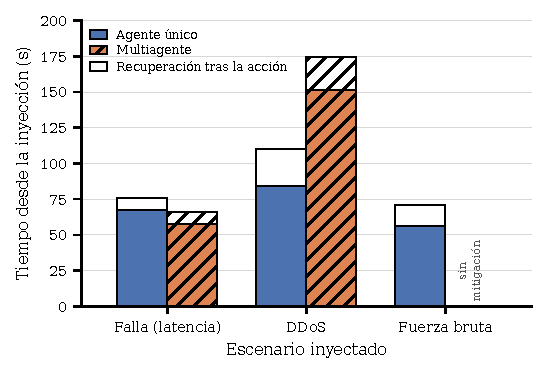
\includegraphics[width=\columnwidth]{fig/mttr_breakdown.pdf}}
\caption{Tiempo medio hasta la primera acción (sólido) y recuperación posterior del
servicio (blanco) por escenario y condición. El total de cada barra corresponde al
MTTR medido por el monitor independiente. Se indica el número de corridas que aporta
cada celda.}
\label{fig:mttr}
\end{figure}

\begin{table}[htbp]
\caption{Resultados del piloto por escenario y condición ($n=5$ por celda)}
\begin{center}
\footnotesize
\setlength{\tabcolsep}{3.2pt}
\begin{tabular}{@{}llcccc@{}}
\toprule
\textbf{Escenario} & \textbf{Cond.} & \textbf{Clase} & \textbf{Expiró} &
\textbf{TTD} & \textbf{MTTR} \\
 & & \textbf{OK} & \textbf{300 s} & \textbf{(s)} & \textbf{(s)} \\
\midrule
Falla        & multi  & 3/5 & 0 & 129.1 & 124.4 \\
Falla        & único  & 3/5 & 2 & ---   & 121.4 \\
DDoS         & multi  & 3/5 & 3 & 182.7 & 121.3 \\
DDoS         & único  & 1/5 & 3 & ---   & 99.7 \\
Fuerza bruta & multi  & 5/5 & 0 & 50.8  & 91.3 \\
Fuerza bruta & único  & 2/5 & 3 & ---   & 70.9 \\
Normal       & multi  & 5/5 & 0 & ---   & --- \\
Normal       & único  & 1/5 & 3 & ---   & --- \\
\midrule
\textbf{Total} & \textbf{multi} & \textbf{16/20} & \textbf{3} & & \\
\textbf{Total} & \textbf{único} & \textbf{7/20}  & \textbf{11} & & \\
\bottomrule
\multicolumn{6}{l}{\scriptsize TTD observable solo en la condición multiagente. MTTR
promediado} \\
\multicolumn{6}{l}{\scriptsize sobre las corridas con mitigación medible.} \\
\end{tabular}
\label{tab:resultados}
\end{center}
\end{table}

\subsection{Fiabilidad de la ejecución}
La comparación entre las acciones declaradas por el sistema y las registradas en la
bitácora de auditoría reveló discrepancias en 13 de las 40 corridas (32.5\,\%). La
forma más frecuente no fue la esperada: en 8 corridas el sistema ejecutó una o más
acciones sobre la infraestructura sin declararlas en su salida estructurada, mientras
que en 3 corridas declaró acciones que nunca se ejecutaron y en 2 el conjunto
declarado difirió del ejecutado.

Se registraron además cinco acciones aplicadas sobre direcciones no pertenecientes al
origen del ataque: cuatro en la condición de agente único y una en la multiagente.
Tres de ellas ocurrieron durante el escenario normal, en el que no había ataque
alguno que contener, y ninguna fue declarada por el agente. Debe notarse que estas
acciones fueron ejecutadas en corridas cuya tarea expiró sin producir salida: el
sistema actuó sobre el cortafuegos y, sin embargo, no emitió reporte alguno.

Este resultado es relevante desde el punto de vista de ingeniería porque invierte el
supuesto habitual sobre la documentación automática: el reporte de un agente no
constituye evidencia de lo ocurrido, ni siquiera en sentido conservador, dado que
puede omitir acciones efectivamente aplicadas. La auditoría independiente de las
llamadas a herramientas, incorporada como salvaguarda de diseño, fue la única vía por
la que estas discrepancias resultaron observables, lo que concuerda con lo señalado en
la literatura sobre agentes con acceso a herramientas \cite{hu2026, debenedetti2026}.

\subsection{Amenazas a la validez}
El tamaño de muestra es de cinco repeticiones por celda. Los intervalos de confianza
calculados por remuestreo resultan amplios, por lo que las diferencias de tiempo se
reportan como preliminares y no admiten una conclusión estadística. La diferencia en
la tasa de respuesta, en cambio, es de magnitud suficiente (90\,\% frente a 35\,\%)
como para no atribuirse al azar.

El tope de 300 s es una restricción de la plataforma de agentes y no un parámetro del
experimento, cuyo tiempo máximo por salto fue fijado en 900 s. Dado que ese tope
afecta de manera desigual a las dos condiciones, el desempeño del agente único
reportado aquí debe entenderse como el de esa arquitectura bajo dicha restricción y no
como un límite del modelo. Una réplica con un tope mayor o con un modelo de inferencia
más rápida podría arrojar una diferencia menor.

Debe declararse además una amenaza de ajuste a los escenarios. Los prompts de rol
fueron refinados iterativamente durante el desarrollo a partir de corridas de prueba
que emplearon los mismos tipos de escenario que la evaluación. Como medida de control,
los prompts fueron congelados antes de la ejecución del piloto y no fueron modificados
durante ella. Las funciones de memoria persistente, destrezas y búsqueda de sesiones
de la plataforma no fueron utilizadas y cada tarea abrió una sesión nueva, pero no
fueron deshabilitadas de forma explícita en los perfiles.

Se empleó un único modelo local de 9B parámetros sobre un único banco de pruebas, por
lo que los resultados no son extrapolables a otros modelos ni a despliegues reales.
El DDoS inyectado opera en capa de aplicación y no produce respuestas de error, por lo
que no cubre la inundación de capa de transporte, y la mitigación no contempló el
escalamiento de réplicas. La calidad de los reportes fue evaluada mediante
comprobaciones automáticas simples, sin una rúbrica aplicada por evaluadores humanos.
Finalmente, la delegación entre agentes fue sustituida por un relevo externo, de modo
que lo evaluado es la especialización de los agentes y no su autonomía de coordinación.

\section{Conclusiones}
Se implementó y se evaluó Hermes-SOC sobre un banco de pruebas en contenedores
mediante un piloto de 40 corridas. El resultado principal no fue el previsto. La
clasificación diferencial entre falla operativa y ataque demostró ser alcanzable con
un modelo local de 9B parámetros: cuando el sistema respondió, acertó en el 89\,\% de
los casos en la condición multiagente y en el 100\,\% en la de agente único, sin
falsas alarmas en el escenario de operación normal. No obstante, el agente único
respondió en apenas 7 de 20 corridas, frente a 18 de 20 de la cadena multiagente,
porque agotó de forma sistemática el tope de tiempo de la plataforma al resolver las
tres fases en un único contexto. En consecuencia, el aporte de la especialización
multiagente no se manifestó como una reducción del tiempo de mitigación, sino como un
aumento de la tasa de finalización de la tarea.

Un segundo hallazgo concierne a la fiabilidad de la documentación automática. En 13 de
las 40 corridas las acciones declaradas por el sistema no coincidieron con las
registradas por la auditoría, y en 8 de ellas se ejecutaron acciones sobre el
cortafuegos o sobre los servicios que el sistema nunca informó. Por consiguiente, en
un agente con capacidad de ejecución la auditoría independiente de las llamadas a
herramientas no constituye una salvaguarda accesoria, sino el único registro fiable de
lo ocurrido.

Como trabajo futuro se contempla replicar el experimento con un tope de tiempo mayor
para aislar el efecto de la plataforma, incorporar un escenario ambiguo de pico
legítimo de tráfico y una línea base de detección por reglas sin modelo de lenguaje, y
evaluar los reportes mediante una rúbrica aplicada por evaluadores humanos.

\begin{thebibliography}{00}
\bibitem{khayat2025} M. Khayat, E. Barka, M. Adel Serhani, F. Sallabi, K. Shuaib, and H. M. Khater, ``Empowering Security Operation Center With Artificial Intelligence and Machine Learning---A Systematic Literature Review,'' \textit{IEEE Access}, vol. 13, pp. 19162--19197, 2025.
\bibitem{kataria2025} V. Kataria, ``Intelligent Site Reliability Engineering: A Multi-agent LLM Framework for Automated Incident Analysis and Root Cause Determination,'' \textit{Int. J. Intell. Eng. Syst.}, vol. 18, no. 11, pp. 450--466, Dec. 2025.
\bibitem{srinivas2025} S. Srinivas \textit{et al.}, ``AI-Augmented SOC: A Survey of LLMs and Agents for Security Automation,'' \textit{J. Cybersecurity Priv.}, vol. 5, no. 4, p. 95, Nov. 2025.
\bibitem{saju2026} M. H. Saju and A. Azim, ``Toward Autonomous SOC Operations: End-to-End LLM Framework for Threat Detection, Query Generation, and Resolution in Security Operations,'' in \textit{Proc. Mach. Learn. Res., vol. 318, 39th Canadian Conf. Artificial Intelligence}, 2026.
\bibitem{roy2026} J. Roy and S. K. Singh, ``AgentSOC: A Multi-Layer Agentic AI Framework for Security Operations Automation,'' in \textit{Proc. 2026 IEEE 5th Int. Conf. AI in Cybersecurity (ICAIC)}, Feb. 2026, pp. 1--7.
\bibitem{soldani2023} J. Soldani and A. Brogi, ``Anomaly Detection and Failure Root Cause Analysis in (Micro) Service-Based Cloud Applications: A Survey,'' \textit{ACM Comput. Surv.}, vol. 55, no. 3, pp. 1--39, Mar. 2023.
\bibitem{tian2026} Y. Tian, Y. Liu, Z. Chong, Z. Huang, Y. Li, and H.-A. Jacobsen, ``GALA: Graph-Augmented LLM Agents for Root Cause Analysis and Incident Response in Microservices,'' in \textit{Proc. 41st IEEE/ACM Int. Conf. Automated Software Engineering}, Oct. 2026, pp. 55--67.
\bibitem{hmimou2025} Y. Hmimou, M. Tabaa, A. Khiat, and Z. Hidila, ``A Multi-Agent System for Cybersecurity Threat Detection and Correlation Using Large Language Models,'' \textit{IEEE Access}, vol. 13, pp. 150199--150215, 2025.
\bibitem{hu2026} Y. Hu, C. Fan, S. Samyoun, and J. Du, ``Log-To-Leak: Prompt Injection Attacks on Tool-Using LLM Agents via the Model Context Protocol,'' in \textit{Proc. 1st Workshop on Security, Privacy, and Safety of Agentic AI Systems}, Nov. 2026, pp. 49--60.
\bibitem{debenedetti2026} E. Debenedetti \textit{et al.}, ``Defeating Prompt Injections by Design,'' in \textit{Proc. IEEE Conf. Secure and Trustworthy Machine Learning (SaTML)}, 2026.
\end{thebibliography}

\end{document}
